\documentclass{article}

\usepackage{hyperref}
\usepackage{graphicx}
\usepackage{tikz}
\usetikzlibrary{shapes}
\usetikzlibrary{positioning}
\usetikzlibrary{fit}
\usetikzlibrary{arrows}

\usepackage{fullpage}
\usepackage[parfill]{parskip}

\title{PCUTL - Module 3:\\ Covering Claim}
\author{Vincent Knight}
\date{}

\begin{document}

\maketitle

In this short covering claim I will provide an overview to my portfolio and describe how I meet the ILOs.\\

This portfolio contains the following documents (in order):

\begin{itemize}
    \item My response to feedback for Module 2;
    \item ``The design and delivery of a new module within the School of Mathematics with ramifications on what it means to be a mathematics graduate from Cardiff.'' (I will refer to this document as `MA1003doc');
    \item ``Description of spring semester'' (document used for peer review with my mentor);
    \item Marking criteria and guidance notes for student assessments relevant to spring semester;
    \item My mentor's peer review with my response;
    \item ``Description of feedback'' (document used for peer review with Phil Anderson)
    \item Phil Anderson's peer review with my response;
    \item Peter Burnap's peer review with my response;
    \item My peer review of Phil Anderson;
    \item My peer review of Peter Burnap;
    \item A page containing links to all supplementary materials (lesson plans etc...)
    \item ``Understanding the perceptions and factors that influence student engagement with formative assessment in mathematics education.'' (the group project).
    \item Two documents relevant to the group assessment portion of our group project.
\end{itemize}

As for my previous portfolio the bulk of my covering claim serves to summarise my various documents, indicating where the ILOs have been achieved. This is shown diagrammatically in Figure \ref{locationofilos}.

\begin{figure}[htdp]
\begin{center}
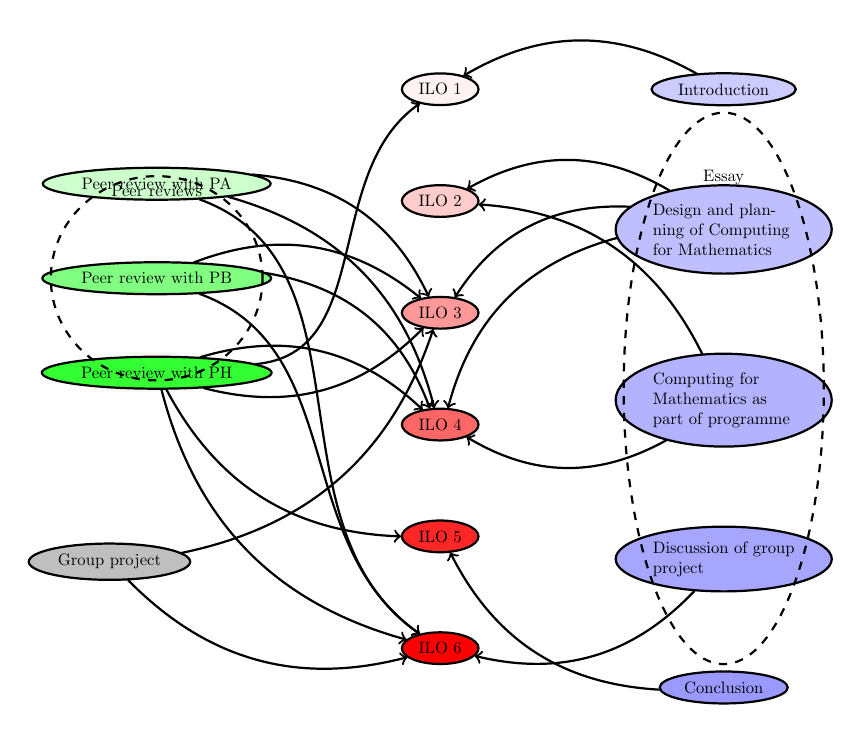
\begin{tikzpicture}[thick,scale=0.6, every node/.style={scale=0.6}]
%------ Listing the ILOs ---------
\node (ILO1) at (0,0) [ellipse, fill=red!5, draw] {ILO 1};
\node [below = 1cm of ILO1] (ILO2) [ellipse, fill=red!20, draw] {ILO 2};
\node [below = 1cm of ILO2] (ILO3) [ellipse, fill=red!40, draw] {ILO 3};
\node [below = 1cm of ILO3] (ILO4) [ellipse, fill=red!60, draw] {ILO 4};
\node [below = 1cm of ILO4] (ILO5) [ellipse, fill=red!85, draw] {ILO 5};
\node [below = 1cm of ILO5] (ILO6) [ellipse, fill=red!100, draw] {ILO 6};

%------ Listing sections of my essay -------
\node (intro) at (6,0) [ellipse, fill=blue!20, draw] {Introduction};
\node [below = 1cm of intro] (design) [ellipse, fill=blue!25, draw, text width=3cm] {Design and planning of Computing for Mathematics};
\node [below = 1cm of design] (programme) [ellipse, fill=blue!30, draw, text width=3cm] {Computing for Mathematics as part of programme};
\node [below = 1cm of programme] (group) [ellipse, fill=blue!35, draw, text width=3cm] {Discussion of group project};
\node [below = 1cm of group] (concl) [ellipse, fill=blue!40, draw] {Conclusion};
\node[fit=(intro)(design)(programme)(group)(concl), ellipse, draw, dashed] (essay) {};
\node [above = -1cm of essay] {Essay};

%----- Peer reviews -------
\node (PA) at (-6,-2) [ellipse, fill=green!20, draw] {Peer review with PA};
\node (PB) at (-6,-4) [ellipse, fill=green!50, draw] {Peer review with PB};
\node (PH) at (-6,-6) [ellipse, fill=green!80, draw] {Peer review with PH};
\node[fit=(PA)(PH), ellipse, draw, dashed] (peerreviews) {};
\node [above = -.35cm of peerreviews] {Peer reviews};

%----- Group project -------
\node (groupproject) at (-7, -10) [ellipse, fill=gray!50, draw] {Group project};

%------ link ILOs ------
\path[<-] (ILO1) edge [bend left] (intro);
\path[<-] (ILO1) edge [out=-145, in=5] (PH);
\path[<-] (ILO2) edge [bend left] (design);
\path[<-] (ILO3) edge [bend left] (design);
\path[<-] (ILO2) edge [bend left] (programme);
\path[<-] (ILO4) edge [bend left] (design);
\path[<-] (ILO3) edge [bend left] (groupproject);
\path[<-] (ILO3) edge [bend right] (PA);
\path[<-] (ILO3) edge [bend right] (PB);
\path[<-] (ILO3) edge [bend left] (PH);
\path[<-] (ILO4) edge [bend right] (programme);
\path[<-] (ILO4) edge [bend right] (PH);
\path[<-] (ILO4) edge [bend right] (PB);
\path[<-] (ILO4) edge [bend right] (PA);
\path[<-] (ILO5) edge [bend right] (concl);
\path[<-] (ILO5) edge [bend left] (PH);
\path[<-] (ILO6) edge [bend right] (group);
\path[<-] (ILO6) edge [bend left] (groupproject);
\path[<-] (ILO6) edge [out=145, in=-20] (PA);
\path[<-] (ILO6) edge [out=145, in=-20] (PB);
\path[<-] (ILO6) edge [bend left] (PH);
\end{tikzpicture}
\end{center}
\caption{Structure of this portfolio}\label{locationofilos}
\end{figure}

There are two main complementary bodies of work in this portfolio:

\begin{itemize}
    \item My essay: MA1003doc;
    \item The group project I participated in.
\end{itemize}

I plan on doing module 4 in the future but nonetheless I feel that completing module 3 marks the end of a journey. Throughout this journey I have been able to identify and place myself as a facilitator of learning within the UK higher education system but also within my school. I have also grown an immense fondness for pedagogic literature and research. Carefully considering state of the art educational methodologies and how they can be incorporated within my own practice has been a strong factor in my PCUTL journey. Finally in this module I feel that I have been able to put a lot of this in practice as I have designed and delivered a brand new module that changes the answer to what it means to be a Cardiff Mathematics graduate.

I cover a range of topics in MA1003doc which is mainly the description of a new module delivered to all single honours first year mathematics students. \textbf{I feel that this essay addresses most of the ILOs of this module but mainly concentrates on ILO 2 and 3 by the fact that I justify the effective module design ensuring efficient and quality learning in line with the appropriate learning outcomes. I give particular attention to the range of learners that will undertake this couse given that I do not want any students to be `left behind' by the pedagic approach: a flipped classroom. The module is designed very much with feedback as a core motivating factor and I discuss this extensively in the essay.}

\begin{itemize}
    \item In the introduction I address ILO 1 by discussing my ongoing activities through the entire PCUTL process (discussing my previous portfolios). This ILO is also addressed throughout my portfolio and MA1003, in particular through my engagement with the literature.
    \item The next section of MA1003doc entitled: `Design and planning of Computing for Mathematics' addresses ILOs 2 and 3, discussing my new module including details with regards the context and the pedagogic approach. Note that I base a lot of what is said in this section on the literature, feedback from students and data from our group project thus ILO 4 is also addressed.
    \item The section entitled `Computing for Mathematics as part of a programme' specifically addresses ILO 2 and 4. As I discuss the place of the new module within the programme at the School of Mathematics (once again basing myself on multi-source data).
    \item I give my thoughts on the group project, specifically discussing how my experience of it will be useful in the delivery of my new module, thus addressing ILO 6.
    \item Finally I conclude this MA1003doc by discussing my plans for further development and engagement with pedagogy (addressing ILO 5). I also comment on the PCUTL process in general.
\end{itemize}

My peer reviews allowed me to address ILO 6 yet again but also ILOs 3 and 4 as I discussed feedback in particular with my peers and the design of my module with Paul. The discussion with my mentor (Paul) was particularly helpful to ensure that my module was placed within the general strategy of the School of Mathematics but also to ensure that the assessment was appropriate. The review of Phil's module design gave me various ideas that I plan on taking forward with my own module (for example details I need to concentrate on when considering speakers for my autumn semester: something I also talked about with Paul). Pete indicated some valuable things to think about with regards to putting in place directives to tutors for future years but also pointed out certain aspects with regards to inclusivity that I need to consider. Such as the potential for students with lesser mobility that cannot take part in role play during my reactive lectures. Furthermore Pete's introductory session that ensures an alignment between student expectation and the ILOs is something I will try and implement in my teaching in the near future.

The original motivation for having two peer reviews with PCUTL colleagues was simply that Pete had not been able to find someone to carry out his peer review with him. On reflection, this was an extremely beneficial thing to do given the untraditional pedagogic approach.  All of my peers (including my mentor Paul) have been very encouraging of my chosen methodology which is reassuring. Furthermore the particular comments and suggestions will all be helpful as I go forward.

In our group project we carried out a rigorous statistical analysis of a questionnaire given to all students studying mathematics within the School of Mathematics and the School of Engineering. The survey allowed us to gain an understanding of student perceptions of formative assessment. This was complimented by a review of the literature. \textbf{This group project obviously allowed me to achieve ILO6 but more importantly aspired to address ILO3. The findings in this group project were taken in to account (and referred to in MA1003doc) in the design of my new module.}

\end{document}
